%!TEX root = ../report.tex
\chapter{Introduction}
\label{ch:context}
This document depicts the software architecture of the Home Energy Monitoring System (HEMS) as the first assignment of Software Patterns course. We proclaim ourself a software architect team working on the Home Energy Monitoring System.

Energy is one of the main concern in a household. The problem is how to monitor energy usage of a particular house in order to prevent inefficient consumption of energy and even to figure out how to save energy, resulting in lower household expenses for energy. An example of energy consumption for a house is shown in Figure \ref{fig:home-energy-consumption}, which indicates that electricity is one of the main energy consumption of a house. Thus, in the initial product this system focuses only on the electricity usage.

\begin{figure}[!ht]
	\centering
	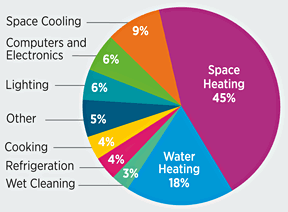
\includegraphics[width=0.35\textwidth]{1-context/images/energysaver_energyuse.png}
	\caption{An example of home energy consumption \cite{greenifynow}.}
	\label{fig:home-energy-consumption}
\end{figure}

This system will allow the user to collect and store their electricity consumption. This system will also have a web dashboard that shows the graph of electricity consumption, which the user can adjust the time range of the graph to see different data, and other useful data such as which device uses the electricity the most, etc. The data, which will be stored in our database, will be used to do analysis that will help user to predict the upcoming electricity bill in the next month and other required analysis. This system also provides a fault-tolerant computing platform to compute these analyses.

The data collection is not our part, we leave this portion of the system to the third party developers. Basically, we provide a service of cloud computing environment, which can be categorized as SaaS\footnote{Software as a service}, to do energy management system. Figure \ref{fig:vision} depicts the architectural vision of the HEMS.

\begin{figure}[H]
	\centering
	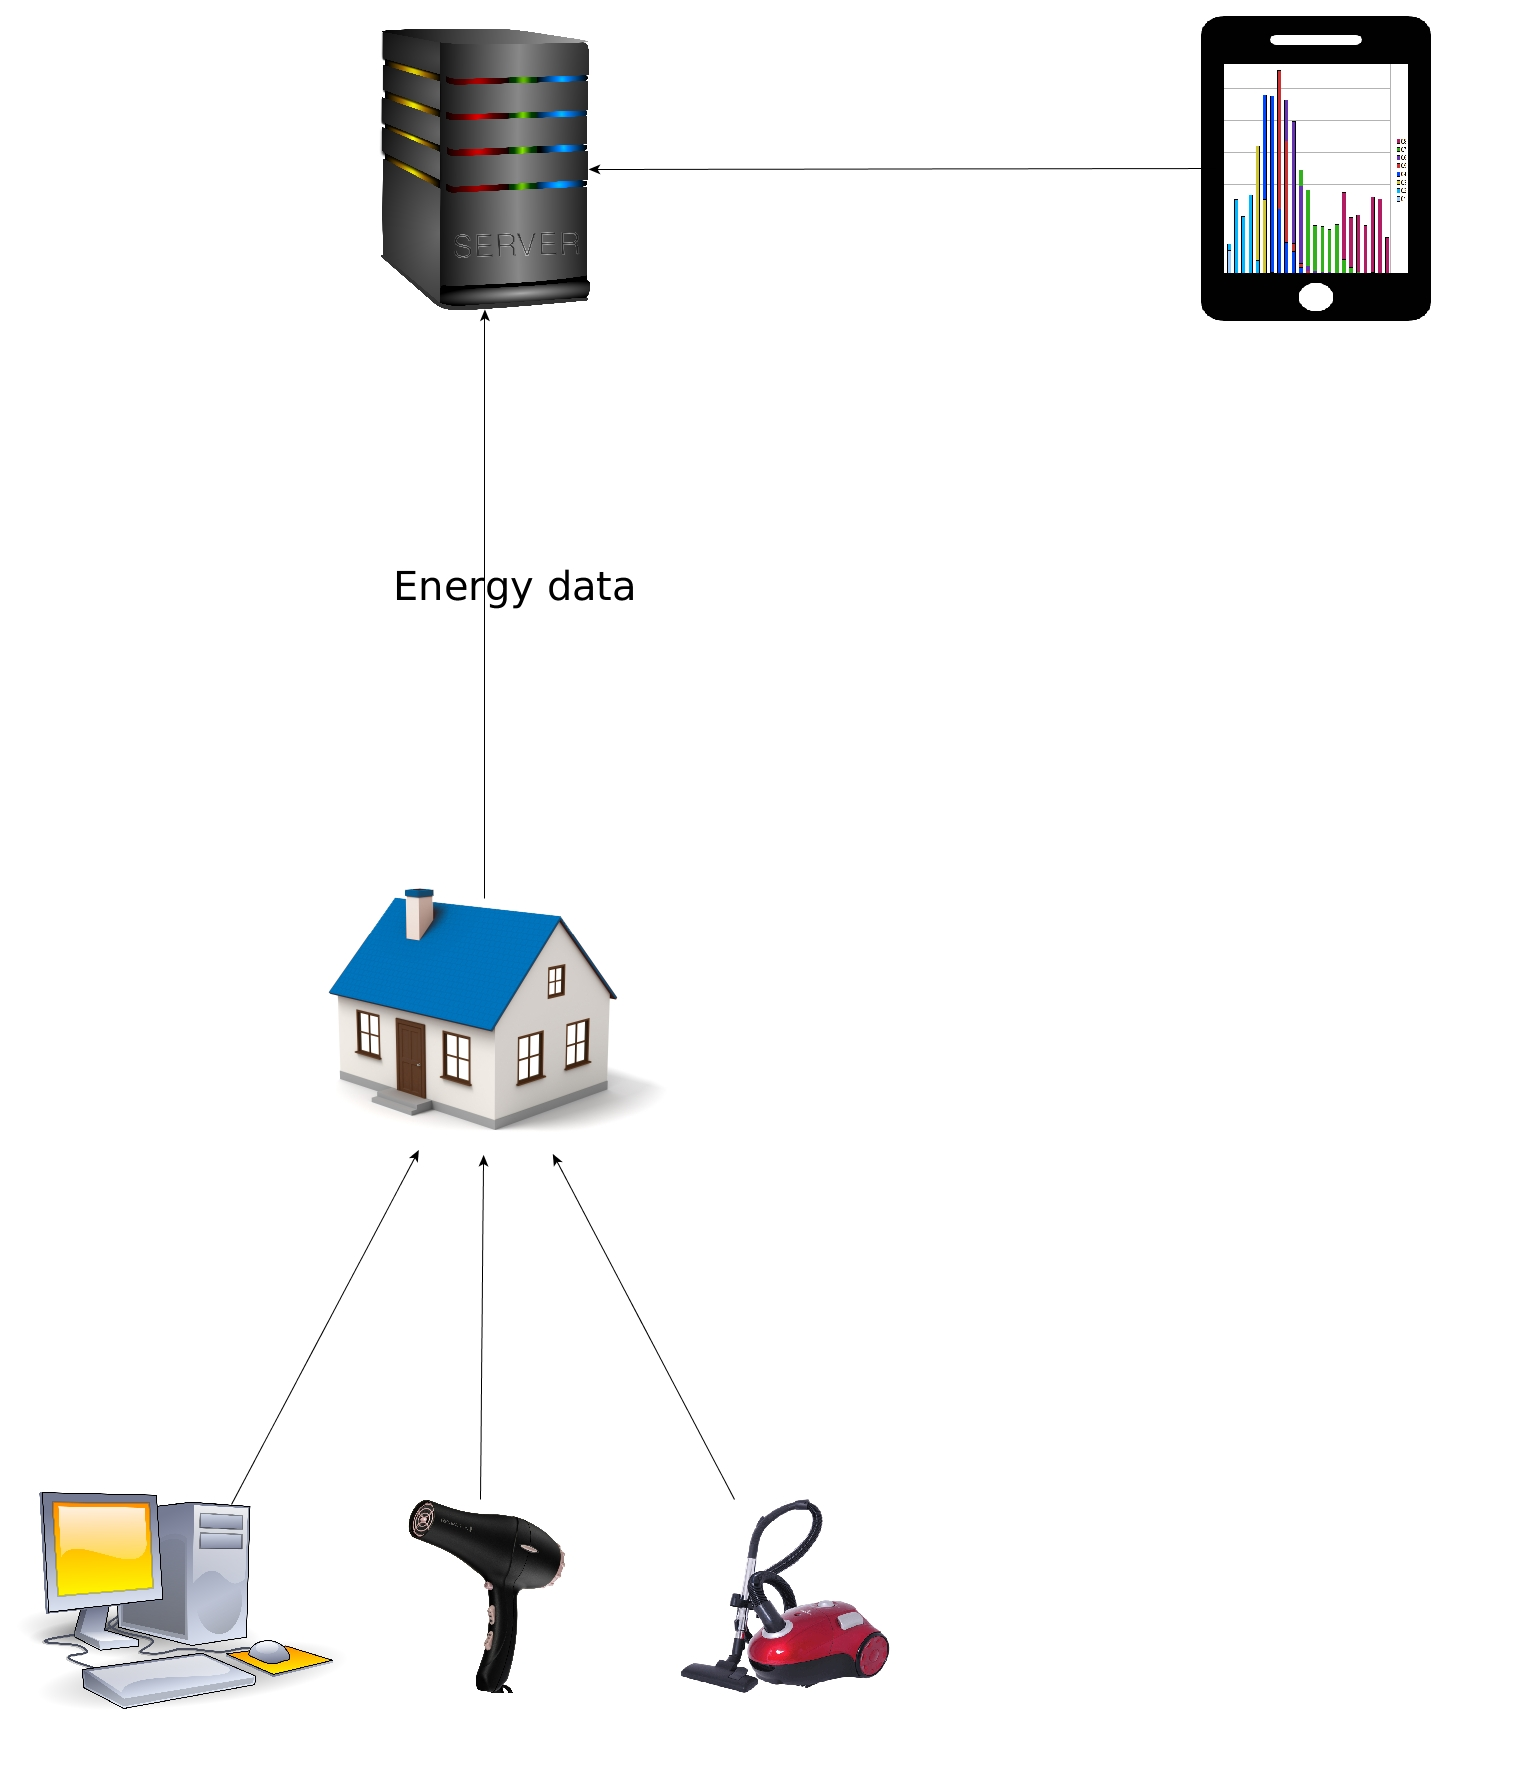
\includegraphics[width=0.5\textwidth]{1-context/images/vision.jpg}
	\caption{Architectural vision}
	\label{fig:vision}
\end{figure}

% \section{System Context} % (fold)
% \label{sec:system_context}
This system provides monitoring for more than one house. Many houses can connect to the system through Internet. Sensors will be located at every device that users are willing to monitor. Real time measurement of electricity consumption will be sent to the HEMS server via Internet protocol by the sensor. Users may see the energy consumption through the web dashboard via computers, tablets, smartphones, or any devices that are able to connect to the Internet.

% Figure \ref{fig:system-context} shows the system context of the HEMS.

% \begin{figure}[!ht]
% 	\centering
% 	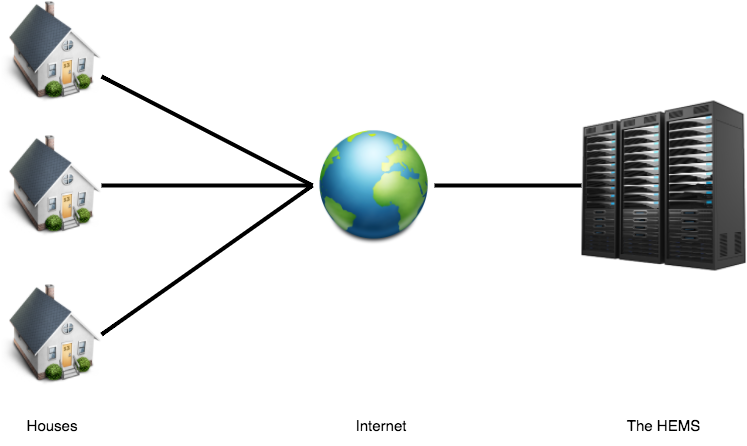
\includegraphics[width=0.7\textwidth]{1-context/images/SP-system-context.png}
% 	\caption{The HEMS system context.}
% 	\label{fig:system-context}
% \end{figure}

The rest of the document is structured as follows. The requirements, use cases, stake holders, and key drivers are explained in chapter \ref{ch:requirements}. Chapter \ref{ch:analysis} describes the analysis and lists the possible pattens to be implemented in this system. Chapter \ref{ch:system} outlines the general system architecture of the system. Hardware selection and architecture are described in chapter \ref{ch:hardware}, while chapter \ref{ch:software} elaborates on software architecture. The evaluation and evolution of this architecture is drawn in chapter \ref{ch:evaluation} and \ref{ch:evolution}. 